\documentclass{article}
\usepackage{graphicx}
\setlength{\oddsidemargin}{0in}
\setlength{\textwidth}{6.5in}
\setlength{\topmargin}{0in}
\setlength{\textheight}{9in}
\begin{document}
\begin{center}
\large\bf Sheba's Amoebas
\end{center}
After a successful Kickstarter campaign, Sheba Arriba has raised
enough money for her mail-order biology supply company.
``Sheba's Amoebas'' can ship Petri dishes already populated with
a colony of those tiny one-celled organisms. However, Sheba
needs to be able to verify the number of amoebas her company sends out.
For each dish she has a black-and-white image that has been
pre-processed to show each amoeba as a simple closed
loop of black pixels. (A loop is a minimal set of black pixels in which
each pixel is adjacent to exactly two other pixels in the set; adjacent means
sharing an edge or corner of a pixel.) All black pixels in the image
belong to some loop. 

Sheba would like you
to write a program that counts the closed loops in a rectangular array
of black and white pixels. 
No two closed loops in the image touch or overlap.
NOTE:
One particularly nasty species of cannibalistic amoeba is known to surround
and engulf its neighbors; consequently there may be amoebas within amoebas.
For instance, each of the figures
below contains four amoebas.

\begin{figure}[htbp]
\centering
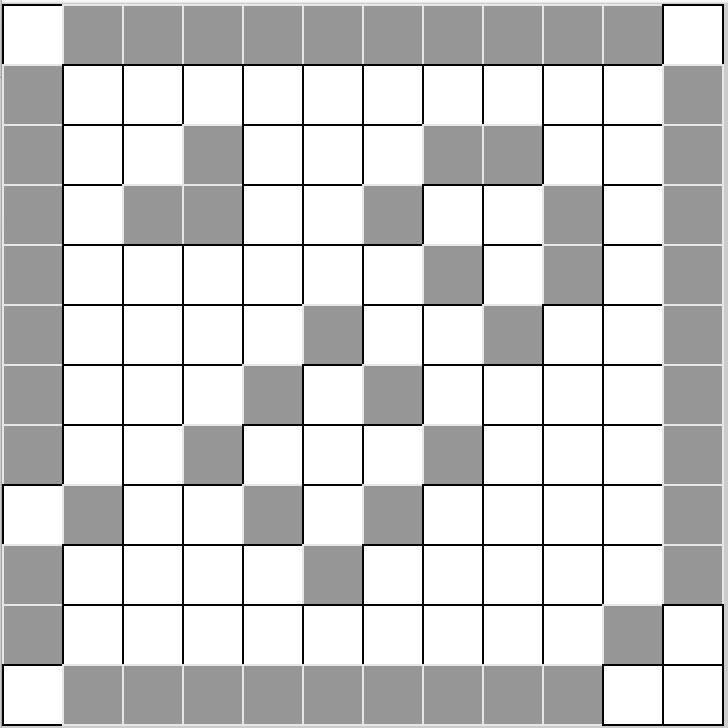
\includegraphics[height=1.5in]{12by12sample}\ \ \ \ \ \ \ \ 
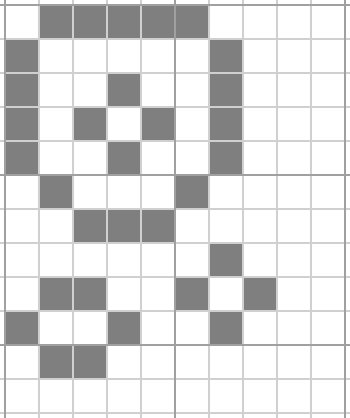
\includegraphics[height=1.5in]{12by10sample}
\end{figure}

\subsubsection*{Input}
The first line contains two integers $m$ and $n$, $1 \leq m,n \leq 100$.
This is followed by $m$ lines, each containing $n$ characters. A
``\verb$#$'' denotes a black pixel, a ``\verb$.$'' denotes a white pixel.

\subsubsection*{Output}
Print a single integer representing the number of loops in the input.

\subsubsection*{Sample Input}
\begin{verbatim}
12 12
.##########.
#..........#
#..#...##..#
#.#.#.#..#.#
#..#...#.#.#
#....#..#..#
#...#.#....#
#..#...#...#
.#..#.#....#
#....#.....#
#.........#.
.#########..
\end{verbatim}
\subsubsection*{Sample Output}
\begin{verbatim}
4
\end{verbatim}
\end{document}
